\documentclass[onepage, 12pt]{beamer}
\mode<presentation>{
	\setbeamercovered{transparent}
	%\beamertemplatenavigationsymbolsempty
	\setbeamertemplate{footline}[frame number]
% 	\usefonttheme{professionalfonts}
}

% https://tex.stackexchange.com/questions/34604/entering-unicode-characters-in-latex
\usepackage[utf8]{inputenc}

% % https://tex.stackexchange.com/questions/446063/change-background-colour-to-black-and-text-to-white
% \usecolortheme{owl}

% https://tex.stackexchange.com/questions/34166/understanding-minipages-aligning-at-top
\usepackage{adjustbox}

% https://tex.stackexchange.com/questions/124256/how-do-i-get-numbered-entries-in-a-beamer-bibliography
\setbeamertemplate{bibliography item}{\insertbiblabel}

% https://tex.stackexchange.com/questions/49048/how-to-cite-one-bibentry-in-full-length-in-the-body-text
\usepackage{bibentry}
\bibliographystyle{plain}
\nobibliography*
%
% https://tex.stackexchange.com/questions/163827/wrong-vertical-spaces-using-bibentry-within-beamer/163842
\def\mybeamernewblock{%
  \usebeamercolor[fg]{bibliography entry author}%
  \usebeamerfont{bibliography entry author}%
  \usebeamertemplate{bibliography entry author}%
  \def\newblock{%
    \usebeamercolor[fg]{bibliography entry title}%
    \usebeamerfont{bibliography entry title}%
    \usebeamertemplate{bibliography entry title}%
    \def\newblock{%
      \usebeamercolor[fg]{bibliography entry location}%
      \usebeamerfont{bibliography entry location}%
      \usebeamertemplate{bibliography entry location}%
      \def\newblock{%
        \usebeamercolor[fg]{bibliography entry note}%
        \usebeamerfont{bibliography entry note}%
        \usebeamertemplate{bibliography entry note}}}}%
  \leavevmode
}
\newenvironment{references}{\begin{itemize}\let\newblock\mybeamernewblock}{\end{itemize}}


\setbeamersize{text margin left=10pt, text margin right=10pt}
\setbeamertemplate{itemize items}[circle]

\beamertemplatenavigationsymbolsempty

% http://tex.stackexchange.com/questions/8680/how-can-i-insert-a-newline-in-a-framebox
%\usepackage{minibox}
%\usepackage{framed}
%\usepackage[usestackEOL]{stackengine}

% https://tex.stackexchange.com/questions/433450/how-to-frame-any-environment-like-minipage-and-others
\usepackage{framed}

% % https://tex.stackexchange.com/questions/91124/itemize-removing-natural-indent
% \usepackage{enumitem}

% % http://tex.stackexchange.com/questions/167000/annotating-tables-with-tikz-adding-arrows
% \usepackage{color, colortbl}
\usepackage{tikz}
\tikzstyle{every picture}+=[remember picture]
%\usetikzlibrary{tikzmark, positioning, fit, shapes.misc}

%% http://tex.stackexchange.com/questions/91124/itemize-removing-natural-indent
%\usepackage{enumitem}

%% http://tex.stackexchange.com/questions/41408/a-five-level-deep-list
%\usepackage{enumitem}
%\setlistdepth{9}

% https://tex.stackexchange.com/questions/20792/how-to-superimpose-latex-on-a-picture
\usepackage{overpic}

% % http://tex.stackexchange.com/questions/32661/how-to-locate-figures-with-x-y-specified-location-in-a-presentation
% \usepackage[absolute,overlay]{textpos} % absolute positioning of stuff
% \setlength{\TPHorizModule}{1mm}
% \setlength{\TPVertModule}{1mm}

\usepackage{graphicx}
\graphicspath{{../img/}}
\AtBeginDocument{\DeclareGraphicsExtensions{.eps, .png, .gif, .pdf, .jpg}}

\usepackage[makeroom]{cancel}

\usepackage[english]{babel}
\usepackage[T1]{fontenc}
\usepackage{times}



% \usepackage{amssymb}
% \usepackage{nicefrac}
% \usepackage{bbm}
% \usepackage{esint}
% \usepackage{sidecap}

\usepackage{hyperref}
% \hypersetup{pdfpagemode=FullScreen}

\newcommand{\HIDE}[1]{}

\newcommand{\skipline}{{\ }\\}

\author{RA}
\subject{Talks}

\newcommand{\CITE}[1]{{\footnotesize[#1]}}

% \input{definitions}

\providecommand{\DIV}{\mathop{\text{div}}}
\providecommand{\GRAD}{\mathop{\text{grad}}}

\providecommand{\IE}{\mathbb{E}}
\providecommand{\IP}{\mathbb{P}}
\providecommand{\IR}{\mathbb{R}}
\providecommand{\IZ}{\mathbb{Z}}

\providecommand{\duality}[2]{\langle #1 \rangle_{#2}}
\providecommand{\norm}[2]{\| #1 \|_{#2}}
\providecommand{\seminorm}[2]{| #1 |_{#2}}
\providecommand{\VERT}{\ensuremath{| \! | \! |}}
\newcommand{\tnorm}[2]{\VERT{#1}\VERT_{{#2}}}

\newcommand{\cA}{\mathcal{A}}
\newcommand{\cB}{\mathcal{B}}
\newcommand{\cL}{\mathcal{L}}
\newcommand{\cN}{\mathcal{N}}
\newcommand{\cT}{\mathcal{T}}
\newcommand{\cX}{\mathcal{X}}
\newcommand{\cY}{\mathcal{Y}}

\providecommand{\Abf}{\mathbf{A}}
\providecommand{\Bbf}{\mathbf{B}}
\providecommand{\Dbf}{\mathbf{D}}
\providecommand{\Ibf}{\mathbf{I}}
\providecommand{\Jbf}{\mathbf{J}}
\providecommand{\Fbf}{\mathbf{F}}
\providecommand{\Hbf}{\mathbf{H}}
\providecommand{\Mbf}{\mathbf{M}}
\providecommand{\Tbf}{\mathbf{T}}
\providecommand{\Pbf}{\mathbf{P}}
\providecommand{\Vbf}{\mathbf{V}}
\providecommand{\pbf}{\mathbf{p}}
\providecommand{\ubf}{\mathbf{u}}
\providecommand{\vbf}{\mathbf{v}}
\providecommand{\wbf}{\mathbf{w}}
\providecommand{\ybf}{\mathbf{y}}
\providecommand{\zbf}{\mathbf{z}}

\renewcommand{\vec}[1]{\mathbf{#1}}

\newcommand{\from}{\colon}

\providecommand{\T}{\mathsf{T}}

\renewcommand{\hat}[1]{\widehat{#1}}
\renewcommand{\tilde}[1]{\widetilde{#1}}

\newcommand{\rd}{\,\mathrm{d}}

\newcommand{\TEXT}[1]{\quad\text{#1}\quad}

% http://tex.stackexchange.com/questions/211518/beamer-vfill-and-itemize
\def\Bottom#1{\vskip 0pt plus 1filll #1}
\def\BottomRight#1{\Bottom{\hfill #1}}

% CODE LISTING
\usepackage{color}
\definecolor{DarkBlue}{rgb}{0,0,0.4}
\definecolor{DarkRed}{rgb}{0.3,0,0}
\definecolor{DarkGreen}{rgb}{0,0.3,0}
\usepackage{listings}
\lstset{%
	language=Python,
	basicstyle=\bf\ttfamily\footnotesize,
	keywordstyle=\color{DarkBlue},
	numbers=left, numberstyle=\footnotesize, numbersep=4pt,
	commentstyle={\color{DarkGreen}},
% 	backgroundcolor=\color{white},
	showspaces=false, showstringspaces=false, showtabs=false,
	frame=none,
	tabsize=4,
	breaklines=true, breakatwhitespace=false,
	emphstyle={[1]\color{blue}},
	emphstyle={[2]\color{DarkGreen}},
	%morekeywords={parfor,true,false},
	xleftmargin=8pt,
	numbers=none
}


%%%%%%%%%%%%%%%%%%%%%%%%%%%%%%%%%%%%%%%%%%%%%%%%%%%%%%%%%%%%%%%%%%%%%%%%%%%%%%%%
%%
%%%%%%%%%%%%%%%%%%%%%%%%%%%%%%%%%%%%%%%%%%%%%%%%%%%%%%%%%%%%%%%%%%%%%%%%%%%%%%%%

\usepackage{ifthen}

\newcommand{\REDBOX}[1]{
	\setlength{\fboxrule}{1pt}
	\fcolorbox{red}{SeeMeBarely}{$\displaystyle
		#1
	$}
}

\definecolor{SeeMeBarely}{RGB}{230,230,230}
\definecolor{Purple}{RGB}{128,0,128}
\definecolor{DeepPurple}{RGB}{32,0,96}
\newcommand{\ra}[1]{{\color{blue}{#1}}}
\newcommand{\cred}[1]{{\color{red}{#1}}}
\newcommand{\cblu}[1]{{\color{blue}{#1}}}
\newcommand{\cpur}[1]{{\color{Purple}{#1}}}

\DeclareMathOperator*{\argmin}{arg\,min}

\newcommand{\ItemComment}[1]{\hfill{\scriptsize(#1)\normalsize}}


% http://www.webnots.com/vibgyor-rainbow-color-codes/
\definecolor{a}{RGB}{148, 0, 211}
\definecolor{b}{RGB}{75, 0, 130}
\definecolor{c}{RGB}{0, 0, 255}
\definecolor{d}{RGB}{0, 160, 0}
\definecolor{e}{RGB}{200, 200, 0}
\definecolor{f}{RGB}{255, 127, 0}
\definecolor{g}{RGB}{255, 0, 0}
%
\definecolor{z}{RGB}{0, 0, 0}
\definecolor{w}{RGB}{255, 255, 255}

% % http://tex.stackexchange.com/questions/17611/how-does-one-type-chinese-in-latex
% \usepackage{CJKutf8}
% \AtBeginDvi{\input{zhwinfonts}}
% %
% \newcommand{\REN}{\begin{CJK*}{UTF8}{gbsn}人\end{CJK*}}
% \newcommand{\ren}[1]{{\color{#1}\REN}}



%%%%%%%%%%%%%%%%%%%%%%%%%%%%%%%%%%%%%%%%%%%%%%%%%%%%%%%%%%%%%%%%%%%%%%%%%%%%%%%%
\begin{document}
%%%%%%%%%%%%%%%%%%%%%%%%%%%%%%%%%%%%%%%%%%%%%%%%%%%%%%%%%%%%%%%%%%%%%%%%%%%%%%%%
%%%%%%%%%%%%%%%%%%%%%%%%%%%%%%%%%%%%%%%%%%%%%%%%%%%%%%%%%%%%%%%%%%%%%%%%%%%%%%%%


\begin{frame}[plain,t]
	\begin{center}
        \vspace{1cm}
		%\small
		%
		Abject mismatch tester gets us
		\\
		{\small\color{gray} Masterclass -- session IV}
		%
% 		\\[1\baselineskip]
% 		\small
% 		RA
% 		\\[1\baselineskip]
% 		\footnotesize
% 		\EMAIL

		\vspace{1cm}
		%

	\end{center}
	
	
	\Bottom{
		\scriptsize
		R.A.
		\hfill
		BSM, Oct 3, 2019
		\\ {\ }
	}
\end{frame}


%%%%%%%%%%%%%%%%%%%%%%%%%%%%%%%%%%%%%%%%%%%%%%%%%%%%%%%%%%%%%%%%%%%%%%%%%%%%

\begin{frame}[t, fragile]{Practice test by Ch.~Rambo}{}

    
    \begin{itemize}
    \item
        \href{http://www.rambotutoring.com/GREpractice.pdf}{www.rambotutoring.com/GREpractice.pdf}
    \item
        \href{http://www.rambotutoring.com/GREpracticeanswers.pdf}{www.rambotutoring.com/GREpracticeanswers.pdf}
        
        {\ }
        \tiny
        
\hfill
%
\begin{minipage}[t]{0.2\textwidth}
\begin{verbatim}
1. B
2. A
3. A
4. E
5. D
6. C
7. C
8. B
9. D
10. D
11. A
12. B
13. B
14. B
15. A
16. B
17. E
18. D
19. B
20. C
21. C
22. A
\end{verbatim}
\end{minipage}
%
\begin{minipage}[t]{0.2\textwidth}
\begin{verbatim}
23. A
24. D
25. D
26. C
27. C
28. E
29. C
30. D
31. D
32. D
33. E
34. A
35. A
36. C
37. E
38. A
39. E
40. C
41. B
42. D
43. A
44. D
\end{verbatim}
\end{minipage}
%
\begin{minipage}[t]{0.2\textwidth}
\begin{verbatim}
45. A
46. E
47. E
48. A
49. D
50. A
51. E
52. D
53. E
54. C
55. A
56. C
57. C
58. B
59. B
60. D
61. C
62. A
63. E
64. A
65. C
66. B
\end{verbatim}
\end{minipage}
%
\hfill
%
{\ }


    \end{itemize}
\end{frame}

%

\begin{frame}[t]{ODE practice}{}
    \begin{minipage}[t]{0.49\textwidth}
        Solve:
        \begin{itemize}
        \item
            $\dot{x}(t) = t \, x(t)$
        \item
            $\dot{x}(t) = t / x(t)$
        \item
            $\dot{x}(t) = x^2(t)$
        \item  
            $\dot{x}(t) = \sqrt{ x(t) }$
        \item
            $\dot{x}(t) = (1 + t^2) (1 + x^2(t))$
        \item
            $\dot{x}(t) = x(t) \log x(t)$
        \item
            $\dot{x}(t) = g(t) h(x(t))$
        \item
            $\dot{x}(t) = a(t) x(t) + b(t)$
        \item
            $\dot{x}(t) = x(t) - x^\alpha(t)$
        \end{itemize}
    \end{minipage}
    %
    \hfill
    %
    \begin{minipage}[t]{0.49\textwidth}
        Tumor models:
        \begin{itemize}
        \item 
            $\dot{V} = a V$
            \hfill
            {\scriptsize(Exponential)}
        \item
            $\dot{V} = a V^b$
            \hfill
            {\scriptsize(Mendelsohn)}
        \item
            $\dot{V} = a V (1 - \frac1b V)$
            \hfill
            {\scriptsize(Logistic)}
        \item
            $\dot{V} = a V \, (b + V)^{-1}$
            \hfill
            {\scriptsize(Linear)}
        \item
            $\dot{V} = a V \, (b + V)^{-1/3}$
            \hfill
            {\scriptsize(Surface)}
        \item
            $\dot{V} = a V \log \frac{b}{c + V}$
            \hfill
            {\scriptsize(Gompertz)}
        \item
            $\dot{V} = a V^{2/3} - b V$
            \hfill
            {\scriptsize(Bertalanffy)}
        \end{itemize}
        
        What is
        \begin{itemize}
        \item 
            the maximal $V$?
        \item
            the condition for growth?
        \item
            the doubling time?
        \end{itemize}
    \end{minipage}
    
    \Bottom{\footnotesize(Various sources)}
\end{frame}

%

\begin{frame}[t]{}{}
    \begin{itemize}
    \item 
        $\cos(y) - \frac{dy}{dx}x \sin(y) + \frac{dy}{dx}y^2 = 0$
    \item
        $\frac{dy}{dx} = \frac{x^2-x+y^2}{e^y-2xy}$
    \item
        $\frac{dy}{dx} + e^{3x} - 4y = 0$
    \item
        $x \frac{dy}{dx} + (x+1)y = 3 \quad (x<0)$
    \item
        $\frac{dy}{dx} = 1 - \frac{y}{x}$
    \item
        $\frac{dy}{dx} = \frac{y-x}{y+x} \quad (x>0)$
    \item
        $y''-y' -12y = 0$
    \item
        $y'' - 4y' + 9y = 0$
    \item
        $y''-6y'+9y = 0$
    \item
        $y''-5y' +6y = 3x + 3$
    \item 
        $y''-5y' +6y = e^{4x}$
    \item
        stability of equilibria of $\frac{dP}{dt} = P(P-5)(P-7)$
    \end{itemize}
    
    \hfill
    {\footnotesize Problems by C.~Tompkins}
\end{frame}

%

\begin{frame}[t]{Information percolation model}{}

    Let $g(x, t)$ denote the cross-sectional 
    density of posterior type $x$
    in the population at time $t$.
    The initial density $g(\cdot, t)$
    of types is given.
    Then
    \begin{align}
        \partial_t g(x, t)
        =
        -\lambda g(x, t)
        +
        \lambda \int_{-\infty}^{\infty}
        g(y, t) g(x - y, t) dy
    \end{align}
    with 
    the first term representing 
    the rate of emigration 
    from type $x$
    associated with meeting and leaving that type,
    and 
    the second term representing
    the rate of immigration
    into type $x$
    due to ``$y$'' meeting ``$x - y$'',
    converting $y$ to $x$.

    \begin{itemize}
    \item 
        Show conservation of (probability) mass.
    \item
        Solve formally and interpret.
    \end{itemize}

    \Bottom{%
        \footnotesize
        D.~Duffie and G.~Manzo, Information percolation in large markets, AER, 2007
    }
\end{frame}

%

\begin{frame}[t]{Goodwin's cyclical macroeconomic model}{}

    Setup:
    \begin{itemize}
    \item 
        (output per annum $Y$) = (capital stock $K$) / (accelerator $\nu$)
    \item
        (employment $L$) = (output $Y$) / (productivity $a$)
    \item
        (employment rate $\lambda$) = (employment $L$) / (population $N$)
    \item
        $\frac{d}{dt} \log$(real wages $w$)
        =
        $(-c + d \times \text{(employment rate $\lambda$)})$
    \item
        (profits $\Pi$) = (output $Y$) - (total wages $w L$)
    \item
        (investment $I$) = (profits $\Pi$)
    \item
        $\frac{d}{dt}$(capital $K$)
        =
        (investment $I$) - (depreciation $\gamma K$)
    \item
        productivity growth: $\alpha$ $\times$ 100\% per annum
    \item
        population growth: $\beta$ $\times$ 100\% per annum
    \end{itemize}
    
    Find a conserved quantity.
    
    \Bottom{%
        \footnotesize
        S.~Keen,
        A monetary Minsky model of the Great Moderation and Great Recession, 
        JEBO, 2013
    }
\end{frame}

%

\begin{frame}[t]{Proabability bits}{}
    The first passenger boarding a plane takes a random seat.
    %
    Then each passenger takes their seat if available;
    otherwise a random seat.
    %
    What is the probability that the last
    passenger gets the right seat?
    
    {\ }
    
    There is a fair and an unfair die/dice.
    %
    The unfair dice shows [$\bullet$] with probability 1/2.
    %
    You take one and throw three [$\bullet$] in a row.
    %
    How likely
    is the same to happen with the other dice?
    
    {\ }
    
    You apply to $n$ different grad schools
    but seal the envelopes before 
    writing the addresses -- randomly. 
    What happens?
    
    {\ }
    
    If the first time I get ``heads'' with a fair coin is on the N-th throw,
    you get N\$.
    %
    Would you play for 2\$?
    
    \Bottom{%
        \footnotesize
        Interview questions, adapted
    }
\end{frame}

%

\begin{frame}[t]{Busybus}{}
    The campus of a small university
    is served by one bus on a circular line.
    %
    From each station ($N = 20$), the bus can go to an adjacent station or stay.
    %
    Meanwhile, exactly one person arrives at a random station
    and waits for the bus to go to some other random station.
    %
    Through an app, the destination of every person currently waiting
    anywhere along the route is known.
    %
    The algorithm chooses who will board the bus at the current station
    respecting the bus capacity ($C = 10$).
    %
    The passengers leave the bus as soon as it arrives at their destination.
    
    \begin{minipage}{0.7\textwidth}
        Find an algorithm that is better than \\
        non-adaptive unidirectional driving.
    \end{minipage}
    %
    \begin{minipage}{0.29\textwidth}
        {\ }
        \centering
        \begin{tikzpicture}[thick,scale=0.8, every node/.style={transform shape}]
            \tiny
            \draw[red,thick,dashed] (1,1) circle (1);
            \filldraw[black] (1+0.5,1+0.87) circle (0.1);% node[anchor=north east] {0};
            \filldraw[black] (1+1,1)        circle (0.1);% node[anchor=east]       {1};
            \filldraw[black] (1+0.5,1-0.87) circle (0.1);% node[anchor=south east] {2};
            \filldraw[black] (1-0.5,1-0.87) circle (0.1);% node[anchor=south west] {3};
            \filldraw[black] (1-1,1)        circle (0.1);% node[anchor=west]       {4};
            \filldraw[black] (1-0.5,1+0.87) circle (0.1);% node[anchor=north west] {5};

            \node[anchor=west, inner sep=0pt] (A) at (1+0.5+0.1,1+0.87) {\rotatebox{-45}{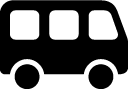
\includegraphics[width=15pt]{bus.png}}};
        \end{tikzpicture}
    \end{minipage}

    \Bottom{%
        \footnotesize
        See also:
        \begin{itemize}
        \item 
            \href{http://bit.do/busybus}{%
                ``Busybus'' coding competition, http://bit.do/busybus, 2017
            }
        \item
            \href{http://bit.do/ac-rep}{%
                A.~Caicedo, \'Etude d'algorithmes pour le probl\`eme du ``Busybus'', 2017
            }
        \end{itemize}
    }
\end{frame}




%%%%%%%%%%%%%%%%%%%%%%%%%%%%%%%%%%%%%%%%%%%%%%%%%%%%%%%%%%%%%%%%%%%%%%%%%%%%%%%%%
%\section{Extra}
%%%%%%%%%%%%%%%%%%%%%%%%%%%%%%%%%%%%%%%%%%%%%%%%%%%%%%%%%%%%%%%%%%%%%%%%%%%%%%%%%
%
%
\newcounter{finalframe}
\setcounter{finalframe}{\value{framenumber}}
% Backup frames follow
%
%
% \begin{frame}
% 	Appendix
% \end{frame}
%
%%
%
%\begin{frame}
%	%
%\end{frame}
%
%
% FINAL SLIDE
\setbeamercolor{background canvas}{bg=black}
\begin{frame}[plain,b]
	\hfill
	\tiny
	\color{gray}
	this slide is intentionally left blank
\end{frame}
\setbeamercolor{background canvas}{bg=white}


%%%%%%%%%%%%%%%%%%%%%%%%%%%%%%%%%%%%%%%%%%%%%%%%%%%%%%%%%%%%%%%%%%%%%%%%%%%%%%%%%
%\section{Bibliography}
%%%%%%%%%%%%%%%%%%%%%%%%%%%%%%%%%%%%%%%%%%%%%%%%%%%%%%%%%%%%%%%%%%%%%%%%%%%%%%%%%

% {
% \tiny
% \bibliography{../../../r/refs}
% }


%%%%%%%%%%%%%%%%%%%%%%%%%%%%%%%%%%%%%%%%%%%%%%%%%%%%%%%%%%%%%%%%%%%%%%%%%%%%%%%%
\setcounter{framenumber}{\value{finalframe}}
\end{document}
%%%%%%%%%%%%%%%%%%%%%%%%%%%%%%%%%%%%%%%%%%%%%%%%%%%%%%%%%%%%%%%%%%%%%%%%%%%%%%%%
%%%%%%%%%%%%%%%%%%%%%%%%%%%%%%%%%%%%%%%%%%%%%%%%%%%%%%%%%%%%%%%%%%%%%%%%%%%%%%%%

